%\documentclass[12pt,a4paper,spanish]{report}
%\documentclass[12pt,a4paper,spanish]{report}
\documentclass[12pt,a4paper,spanish]{article}

\usepackage[spanish]{babel}
\usepackage[utf8]{inputenc}
\usepackage[T1]{fontenc}
\usepackage{amsmath}
\usepackage{graphicx}
\usepackage[retainorgcmds]{IEEEtrantools}
\usepackage{fancybox}
%\usepackage{hyperref} % páginas web e hipervínculos en el documento
\usepackage[hidelinks]{hyperref} % no dibuja el recuadro del vínculo
\usepackage[usenames]{color}
\usepackage{xcolor}
\usepackage{enumerate}
\usepackage{amsfonts,amssymb}
\usepackage{xfrac} % para fracciones		    <=== sfrac
%\usepackage[makeroom]{cancel} %para cancelar
%\usepackage{paralist}
%\usepackage{multirow}
\usepackage{fancyhdr}
\usepackage{mathtools} %cuadros en ecuaciones
\usepackage{tcolorbox} % " de color
%\usepackege[table,xcdraw]{xcolor} %se utiliza con
%definecolor{nombre}{HTML}{69A84F} <- color hexadecimal
%\usepackage{datetime}
%
%\usepackage[style=apa]{biblatex}
%\DefineBibliographyStrings{spanish}{andothers={\textit{\!et al.,}}}
%\usepackage{csquotes}

%\usepackage[backend=biber,citestyle=authoryear,bibstyle=authortitle,sorting=nyt]{biblatex}
%\usepackage{natbib}% citas tipo Harvard (autor,año)
%\usepackage[round,comma,authoryear]{natbib}% citas tipo Harvard (autor,año)
%\citestyle{apa}
%\usepackage{apalike}
%\usepackage{biblatex}
%\usepackage[fixlanguage]{babelbib}
%\usepackage{babelbib}
%\usepackage{tasks}    % para listas horizontales    <=== > task(s)
%%\usepackage{exsheets} % para exámenes		      <===

\usepackage{caption}
\captionsetup{font=small,labelfont=bf} %modifica los captions
%\captionsetup[table]{font=small,labelfont=bf} %modifica los captions
%\captionsetup[table]{font=small,labelsep=period,labelfont=bf} %modifica los captions
%\captionsetup[figure]{font=small,labelfont=bf} %modifica los captions
%\captionsetup[longtable]{font=small,labelsep=period,labelfont=bf,width=16.5cm}
%%\usepackage[subfolder]{gnuplottex} % cleanup
\usepackage{keyval,latexsym,ifthen,moreverb} %requerido por caption
\usepackage{listings} % para insertar código
% para figura en primera página
% src: https://tex.stackexchange.com/questions/167719/how-to-use-background-image-in-latex
%\usepackage{tikz}
% src: https://ipfs-sec.stackexchange.cloudflare-ipfs.com/tex/A/question/46280.html
\usepackage{transparent}
%\usepackage{wallpaper}
%\usepackage{eso-pic}
%\newcommand\BackgroundPic{%
%  \put(0,0){%
%  \parbox[b][\paperheight]{\paperwidth}{%
%  \vfill
%  \centering
  %{\transparent{0.4}%
%  \includegraphics[width=\paperwidth,height=\paperheight,%
%  keepaspectratio]{img/tapa.eps}%
  %}
%  \vfill
%  }}}

%============
\newcommand*\rot{\rotatebox{60}}

% para el estilo y forma de la página
\addtolength{\textwidth}{2.5cm}
\pagestyle{fancy}
\lhead{\bf{G32}}
\chead{}
\rhead{\sl Dos Santos, Gramajo, Rubio \& Coca}
\lfoot{\sl AEyCD}
\cfoot{}
\rfoot{\thepage}
\renewcommand{\headrulewidth}{0.5pt}
\renewcommand{\footrulewidth}{0.5pt}
%\linespread{1.11} %separación entre líneas

\textheight 23cm 
%\textwidth 165mm
\topmargin -1cm 
\oddsidemargin 0in
\evensidemargin 0in
%\evensidemargin -1.5in

\def\fecha#1{\sf\large
%  \newcommand\myToday{
    #1 de
    \ifcase\month\or Enero\or Febrero\or Marzo\or Abril\or Mayo\or Junio\or
    Julio\or Agosto\or Septiembre\or Octubre\or Noviembre\or Diciembre\fi\space de
    \number\year
  }

\newcommand\myToday{ 
  \ifcase\month\or Enero\or Febrero\or Marzo\or Abril\or Mayo\or Junio\or
  Julio\or Agosto\or Septiembre\or Octubre\or Noviembre\or Diciembre\fi\space de
  %\space\number\day,  
  \number\year}

% cuadros
\newcommand{\cuadro}[1]{%
%{\begin{center} \ovalbox{\begin{minipage}[c]{.9\textwidth}
{\begin{center} \framebox{\begin{minipage}[c]{.9\textwidth}
 \begin{center} 
    { #1}
  \end{center} \end{minipage} }
 \end{center}}
 }

%
\newcounter{problema}
%
\renewcommand{\baselinestretch}{1.5}
\newcommand{\prob}[1]{\stepcounter{problema} 
\noindent{\bf Problema Nº \arabic{problema}:} }

\newcommand{\probp}[1]{\stepcounter{problema} 
\noindent{\bf Problema Nº \arabic{problema}: {\it(#1 pts.)}} }

% cambio de Listing a Sintáxis
\renewcommand{\lstlistingname}{Sintáxis}


% enumerate environment
% fuente: http://en.wikibooks.org/wiki/LaTeX/List_Structures
%\let\oldenumerate\enumerate
%\renewcommand{\enumerate}{
%  \oldenumerate
%  \setlength{\itemsep}{-5pt}
%  \setlength{\parskip}{0pt}
%  \setlength{\parsep}{0pt}
%}




% redifine item command !!! usar este
%\newlength{\wideitemsep}
%\setlength{\wideitemsep}{.1\itemsep}
%\addtolength{\wideitemsep}{-7pt}
%\let\olditem\item
%\renewcommand{\item}{\setlength{\itemsep}{\wideitemsep}\olditem}

\addto\captionsspanish{%
  \renewcommand{\tablename}%
  {Tabla}
}

% redifine item command
%\newlength{\wideitemsep}
%\setlength{\wideitemsep}{.1\itemsep}
%\addtolength{\wideitemsep}{-7pt}
%\let\olditem\item
%\renewcommand{\item}{\setlength{\itemsep}{\wideitemsep}\olditem}


\makeatletter % para usar con tcolorbox
\let\Asol\Aboxed
\let\@Asol\@Aboxed
\patchcmd{\Asol}{\@Aboxed}{\@Asol}{}{}%
\patchcmd{\@Asol}{\boxed{#1#2}}{\fcolorbox{red}{yellow}{$\displaystyle #1#2$}}{}{}%
\makeatother


%\documentclass[12pt, a4paper, spanish]{article}
%\usepackage{graphicx} % Required for inserting images
\usepackage{rotating}
\usepackage{hyperref}



\title{Diplomatura en Ciencia de Datos, Aprendizaje Automático y sus Aplicaciones \\[5mm]
\Large{Análisis Exploratorio y Curación de Datos}
}
\author{\emph{Daniel Andres Dos Santos, Luciana Gramajo, Natalia Rubio \& Sebastián Coca
}}
\date{\small \myToday}

\begin{document}

\maketitle

\section*{Trabajo práctico entregable 2 - Parte 1}

En este trabajo se analiza el conjunto de datos de la compentencia Kaggle sobre estimación de precios de ventas de propiedades en Melbourne, Australia. 
El objetivo de este análisis es determinar qué variables son significativas en la explicación del precio de las propiedades situadas en Melbourne, Australia con el fin de lograr predecir el valor de una vivienda con determinadas características específicas.
Para ello en una primera instancia se implementaron consultas en SQL que tienen en cuenta la siguiente información:

\begin{itemize}
\item cantidad de registros totales por ciudad.
\item cantidad de registros totales por barrio y ciudad.
\end{itemize}

Se creó una base de datos (archivo `.bd') tanto con los datos de Melbourne y los datos disponibles de Airbnb. Para combinar ambas tablas ingestadas mediante JOIN de SQL usamos la información del código postal que es común a ambas bases de datos (`zipcode' en airbnb y `Postcode' en melb), unificando todos los valores a reales.

Para predecir el valor de la propiedad analizamos el comportamiento tanto de las variables cuantitativas como cualitativas, por lo que se tuvieron que estudiar en una primera aproximación por separado.


\subsection*{Variables cuantitativas}
Se realizó un resumen de las medidas descriptivas de las variables cuantitativas para obtener la información, como se puede ver en la Tabla \ref{t.medidas} y Figura \ref{f1}.


%\begin{landscape}
%#\pagestyle{empty}


\begin{table}[h]
  \small
  \centering
  \caption{Medidas descriptivas de las variables cuantitativas.}
  \label{t.medidas}
  \begin{tabular}{l|rrrrrrrrrrrrr}
  \hline\hline
    & count & mean & std & min & 25\% & 50\% & 75\% & max \\
    \hline
    Rooms & 13580 & 2.9 & 1.0 & 1.0 & 2.0 & 3.0 & 3.0 & 10.0 \\
    
    Price & 13580 & 1.1$\times 10^6$ & 6.4$\times 10^5$ & 8.5$\times 10^4$ & 6.5$\times 10^5$ & 9.0$\times 10^5$ & 1.3$\times 10^6$ & 9.0$\times 10^6$ \\
    
    Distance & 13580 & 10.1 & 5.9 & 0.0 & 6.1 & 9.2 & 13.0 & 48.1 \\
    
    Postcode & 13580 & 3105.3 & 90.7 & 3000.0 & 3044.0 & 3084.0 & 3148.0 & 3977.0 \\
    
    Bedroom2 & 13580 & 2.9 & 1.0 & 0.0 & 2.0 & 3.0 & 3.0 & 20.0 \\
    
    Bathroom & 13580 & 1.5 & 0.7 & 0.0 & 1.0 & 1.0 & 2.0 & 8.0 \\
    
    Car & 13518 & 1.6 & 1.0 & 0.0 & 1.0 & 2.0 & 2.0 & 10.0 \\
    
    Landsize & 13580 & 558.4 & 3990.7 & 0.0 & 177.0 & 440.0 & 651.0 & 433014.0 \\
    
    BuildingArea & 7130 & 152.0 & 541.0 & 0.0 & 93.0 & 126.0 & 174.0 & 44515.0 \\
    
    YearBuilt & 8205 & 1964.7 & 37.3 & 1196.0 & 1940.0 & 1970.0 & 1999.0 & 2018.0 \\
    
    Lattitude & 13580 & -37.8 & 0.1 & -38.2 & -37.9 & -37.9 & -37.8 & -37.4 \\
    
    Longtitude & 13580 & 145.0 & 0.1 & 144.4 & 145.0 & 145.0 & 145.1 & 145.5 \\
    
    Propertycount & 13580 & 7454.4 & 4378.6 & 249.0 & 4380.0 & 6555.0 & 10331.0 & 21650.0 \\
    \hline\hline
  \end{tabular}
\end{table}


\normalsize

\begin{figure} [!ht]
\begin{center}
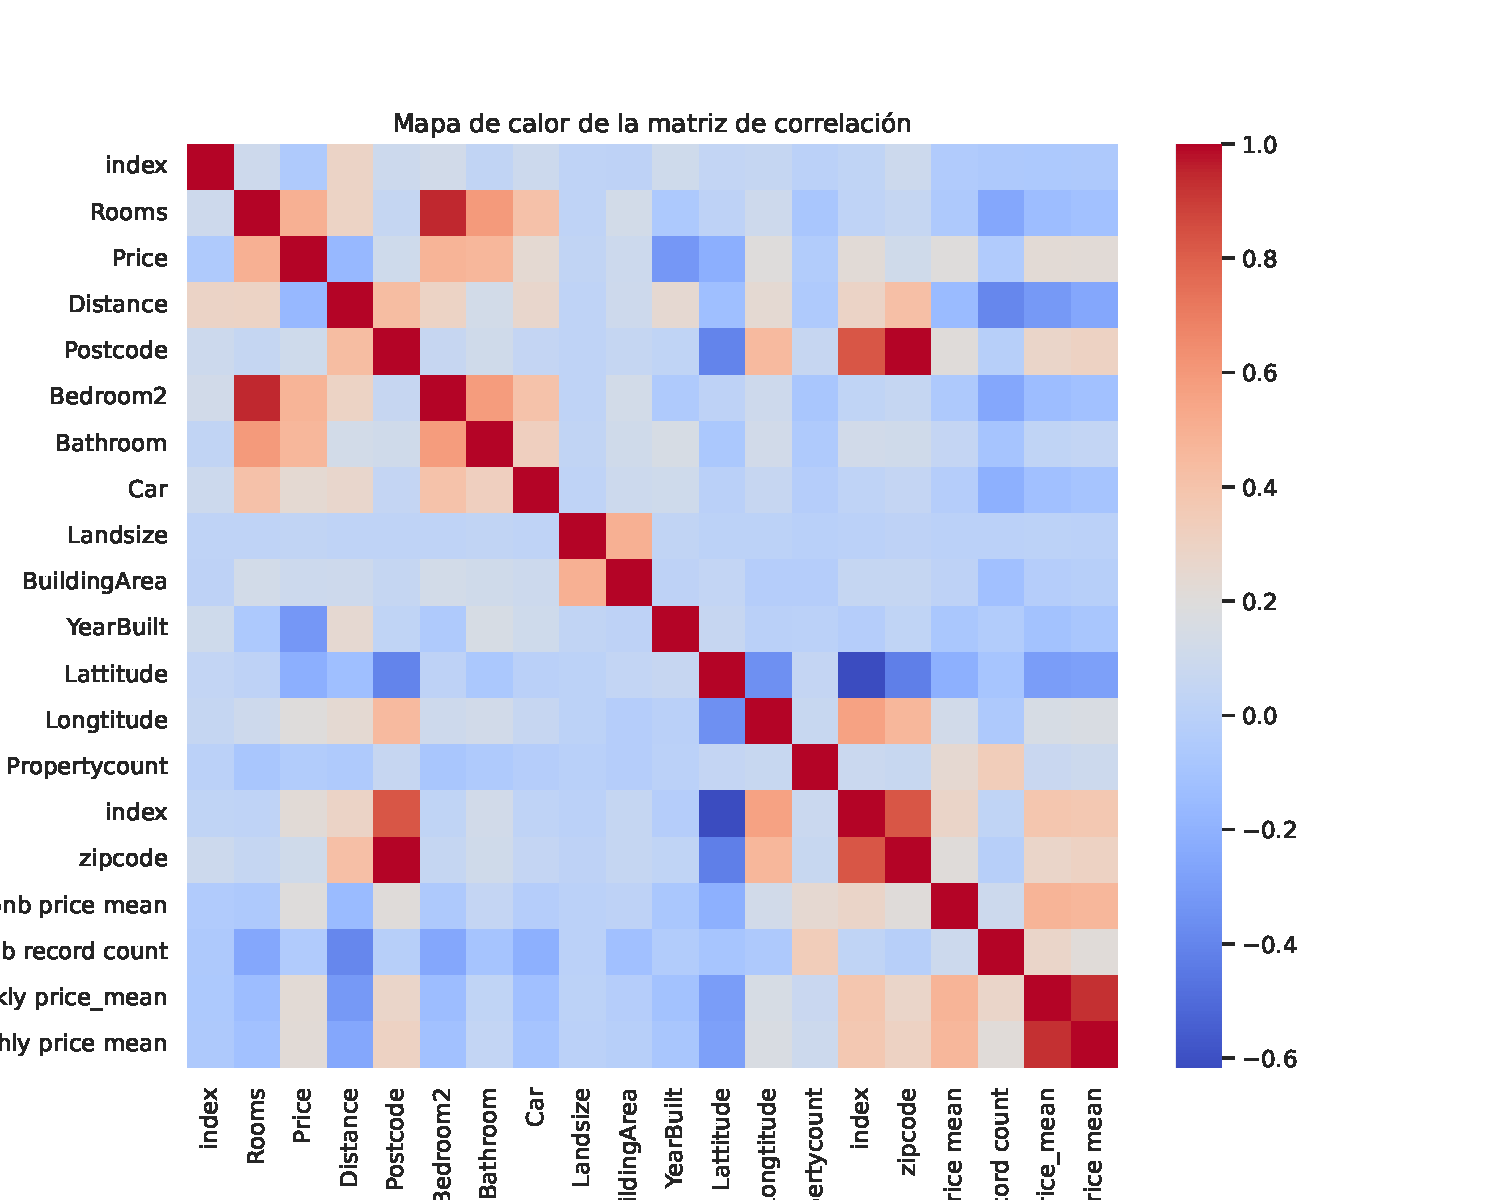
\includegraphics[width=1.0\columnwidth]{img/correlacion.pdf}
\caption{Heatmap de correlación entre las variables numéricas.}
\label{f1}
\end{center}
\end{figure}


En la Tabla \ref{t.medidas} se puede observar el conteo para cada variable, la media, la mediana, la dispersión de los datos, primer y tercer cuartil y el valor máximo para cada variable. Además se puede notar en la misma, en qué variable faltan datos.
A continuación, para realizar una selección de las variables cuantitativas que aportan a la explicación de la variable de respuesta, se calculó el coeficiente de correlación de Pearson (Ver Tabla \ref{t.corr}).
\begin{table} [!ht]
\small
\centering
\caption{Variables que presentan mayor correlación con el Precio.}
    \label{t.corr}
\begin{tabular}{crcr}
\hline\hline
index & -0.054 & \colorbox{cyan}{YearBuilt} & \colorbox{cyan}{-0.324} \\
\colorbox{cyan}{Rooms} & \colorbox{cyan}{0.497}  & \colorbox{cyan}{Lattitude} & \colorbox{cyan}{-0.213} \\
Price & 1.000 & \colorbox{cyan}{Longtitude} & \colorbox{cyan}{0.204} \\
Distance & -0.163 & Propertycount & -0.042 \\
Postcode & 0.108 & index & 0.221 \\
\colorbox{magenta}{Bedroom2} & \colorbox{magenta}{0.476} & zipcode & 0.111 \\
\colorbox{magenta}{Bathroom} & \colorbox{magenta}{0.467} & airbnb price mean  & 0.199 \\
Car & 0.239 & airbnb record count & -0.044 \\
Landsize & 0.038 & airbnb weekly price\_mean & 0.223 \\
BuildingArea & 0.091 & airbnb monthly price mean & 0.221 \\
\hline\hline
\end{tabular}
\end{table}
Podemos observar que las variables que están más correlacionadas son:

\begin{itemize}
\item Tipo de Construcción
\item Cantidad de Ambientes
\item Ubicación: Latitud y Longitud
\item Año de Construcción
\end{itemize}


Cabe aclarar que, la cantidad de los ambientes son una combinación lineal de cantidad de dormitorios y cantidad de baños, por lo tanto estas variables no se incluyen en el análisis. 
También se calcularon las correspondientes correlaciones entre todas las variables cuantitativas para observar si entre las cuantitativas existían correlaciones significativas. Donde se puede corroborar que el Código postal está correlacionado con longitud y latitud lo cual puede estar atribuido a la forma de asignación del código postal de cada vivienda. También se observa que las variables que comentamos anteriormente, cantidad de dormitorios y cantidad de baños, está correlacionada con cantidad de ambientes.
Además, encontramos que entre el año de construcción y el precio la relación que existe es inversa, lo cual sugiere que las viviendas más recientes (o sea, registradas para año calendario más elevado) tienen menor precio que las más antiguas (o sea, registradas en años pretéritos). Resultaría importante indagar con cuáles factores co-varía la edad de una vivienda para dar cuenta de dicho fenómeno (e.g. calidad de materiales, locación geográfica y tamaño). 
Por otro lado, decidimos también mantener la columna de la variable `BuildingArea' dado que la vamos a necesitar en la parte 2 del práctico.

Por lo tanto, como resultado de este primer análisis, se seleccionan las siguientes variables del grupo de variables cuantitativas:

\begin{itemize}
\item Tipo de Construcción
\item Cantidad de Ambientes
\item Ubicación: Latitud y Longitud
\item Año de Construcción
\item Área de construcción
\end{itemize}


\subsection*{Variables Cualitativas o Categóricas}

Para el análisis de las variables categóricas se realizó un análisis análogo al de las variables cuantitativas pero no numérico. Por lo tanto se utilizó el estadístico F, como se presenta en la Tabla \ref{t.f} y un análisis gráfico de las variables seleccionadas (e.g. Figuras \ref{caja1} y \ref{caja2}).

El uso del estadístico F, es para ver cuanto se segrega la variabilidad entre las variables cualitativas. El estadístico F compara la variabilidad entre los grupos con la variabilidad dentro de los grupos. Si el estadístico F es grande y el valor p asociado es menor que un umbral de significancia predefinido (generalmente 0.05), se rechaza la hipótesis nula y se concluye que al menos una de las medias de los grupos es significativamente diferente. En nuestro análisis se seleccionaron entre las variables significativas aquellas que tengan valores mayores y comparables en magnitud de F-scores. Entonces, de estas nos quedaron las variables Tipo de vivienda o  `Type' y Región  o `Regionname'.

\begin{table}[!ht]
\small
\centering
\caption{Valores del estadístico F.}
\label{t.f}
\begin{tabular}{l|r}
\hline\hline
Suburb & 19.3 \\
Address & 2.3 \\
Type & 1409.0 \\
Method & 42.8 \\
SellerG & 14.8 \\
Date & 6.5 \\
CouncilArea & 97.2 \\
Regionname & 284.4 \\
\hline\hline
\end{tabular}
\end{table}

Como se mencionó anteriormente, también realizamos un análisis gráfico mediante Diagrama de Cajas para las variable Precio de la Propiedad según la variable Tipo de Vivienda (Figura \ref{caja1}) y  Región (Figura \ref{caja2}). Además realizamos un scatter plot para cruzar tres variables: habitación (`Rooms'), Precio (`Price') y Año de construcción (`YearBuilt'), como se puede ver en la Figura \ref{amb-anio}. 


\begin{figure} [!ht]
\begin{center}
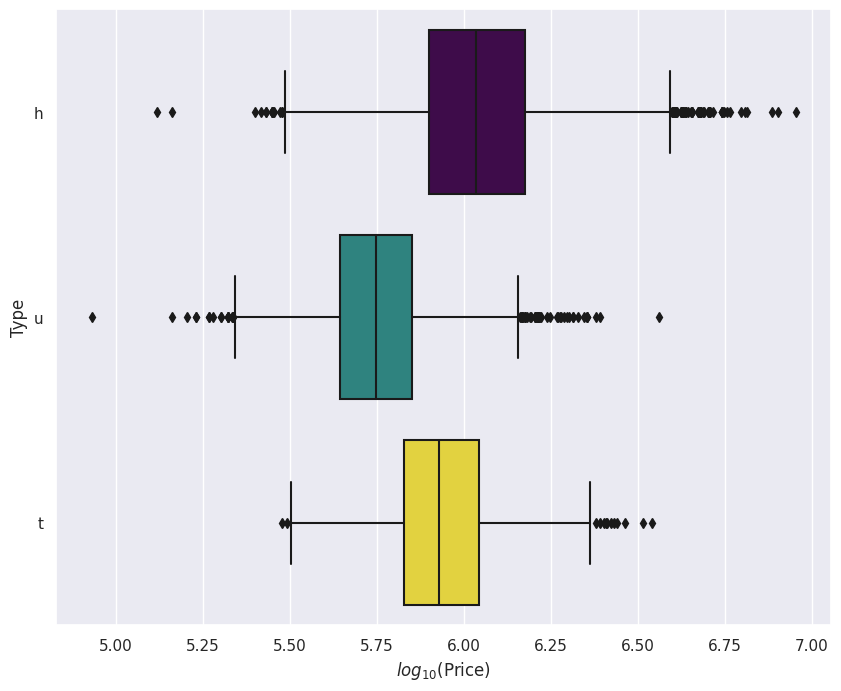
\includegraphics[width=0.8\columnwidth]{img/box1.png}
\caption{Diagrama de Cajas del Tipo de vivienda según el Precio en escala logarítmica.}
\label{caja1}
\end{center}
\end{figure}

En particular, en la Figura \ref{caja1} se representa la distribución del precio para los diferentes tipos de vivienda. Podemos observar que la categoría h, que incluye viviendas tipo casa, cabaña, villa es la que presenta una mayor dispersión y cuenta con más cantidad de puntos extremos. Por otra parte, si analizamos los precios promedios podemos ordenar las categorías de mayor a menor: H(casa) - T (casa adosada) -U (Dúplex), siendo estos últimos los más homogéneos.

\begin{figure} [!ht]
\begin{center}
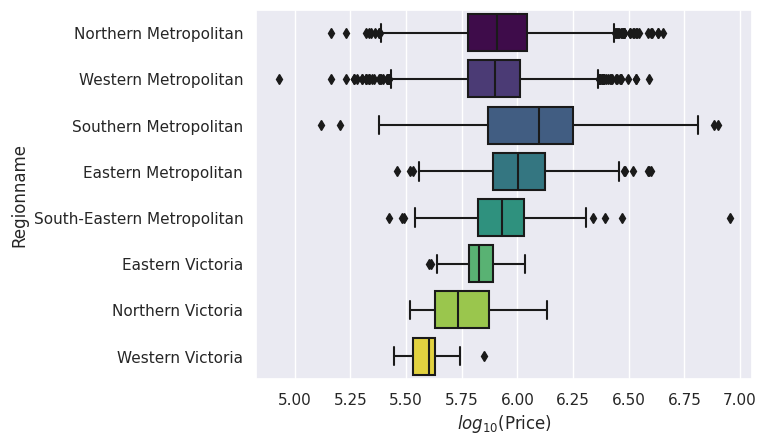
\includegraphics[width=0.8\columnwidth]{img/box2.png}
\caption{Diagrama de Cajas correspondientes a la Región según su Precio en escala logarítmica.}
\label{caja2}
\end{center}
\end{figure}


Si observamos los resultados obtenidos en la Figura \ref{caja2} podemos ver que las viviendas que se encuentra al sur son las mas dispersas y tienen un precio medio mas elevadas que el resto. Por el contrario las que están al Oeste, resultan ser las de menor precio promedio y se encuentran mas concentradas.

\begin{figure} [!ht]
\begin{center}
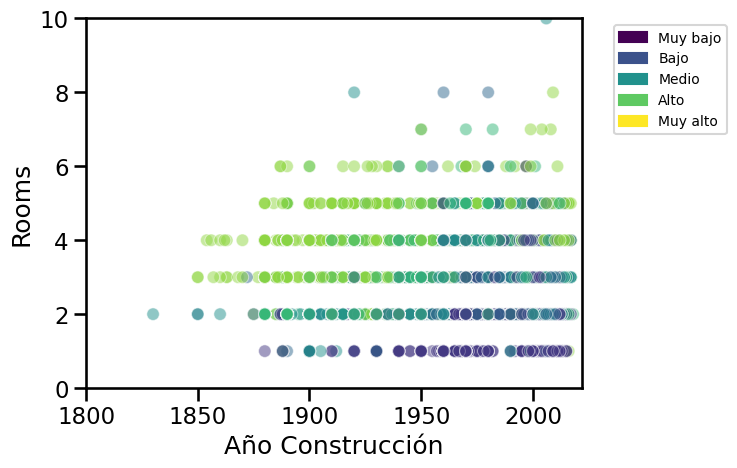
\includegraphics[width=0.8\columnwidth]{img/Scatt1.png}
\caption{Precios de la viviendas según Cantidad de Ambientes y Año de Construcción.}
\label{amb-anio}
\end{center}
\end{figure}

%\clearpage 


Entonces a partir de los resultados obtenidos del análisis cualitativo y cuantitativo seleccionamos las siguientes variables:

\begin{itemize}
\item Tipo de Construcción (Type: br - bedroom(s); h - house, cottage, villa, semi, terrace; u - unit, duplex; t - townhouse; dev site - development site; o res - other residential)
\item Cantidad de Ambientes (Rooms: Number of rooms)
\item Ubicación: Latitud y Longitud (Lattitude y Longtitude) 
\item Año de Construcción (YearBuilt: Year of building dating back hundreds of years in some cases)
\item Area de Construcción (BuildingArea)
\item Región (Regionname)
\end{itemize}




Finalmente, los resultados obtenidos en esta parte del entregable lo guardamos en el archivo: dfjoin.csv. En éste, las columnas seleccionadas son las que potencialmente nos darían la información necesaria para predecir el precio. Decidimos mantener también las columnas provenientes de airbnb además de la columna `BuildingArea' que la vamos a necesitar en la parte 2 del práctico. A los efectos de preservar la información geográfica, se decide conservar el dato de coordenadas geográficas para los registros.



%, y las que nos quedaron son `Type' y `Regionname'.


\subsection*{Eliminación de valores extremos }

Una vez seleccionadas las variables cuantitativas y cualitativas que van a intervenir en la explicación de la variable precio de la vivienda, procedimos a eliminar los valores extremos que no influyen en la estimación a realizar.
Para ello se utiliza el criterio de eliminar las observaciones que están por encima de 1,5 veces del Rango Intercuartilico.
Previamente se transformaron los valores de la variable Precio, a través una transformación logarítmica, para luego analizar si la misma posee una Distribución Normal.

\begin{figure} [!t]
\begin{center}
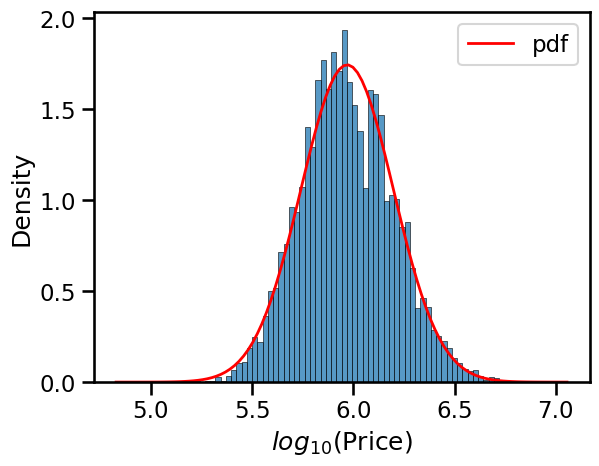
\includegraphics[width=0.7\columnwidth]{img/logprecio.png}
\caption{Distribución de densidad del logarítmo de los Precios de la viviendas.}
\label{Precios}
\end{center}
\end{figure}


\begin{figure} [!ht]
\begin{center}
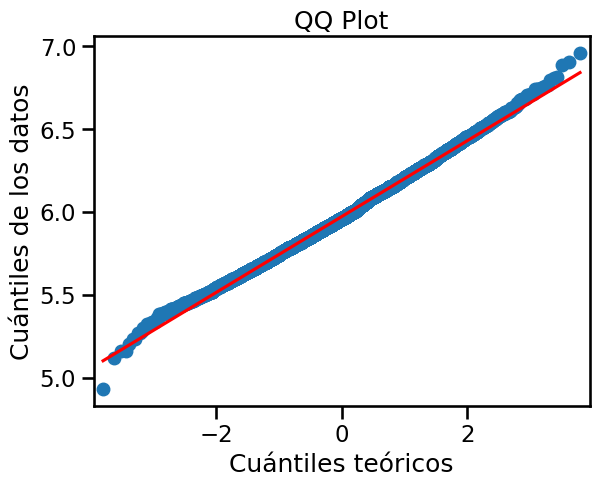
\includegraphics[width=0.7\columnwidth]{img/qqpPrecio.png}
\caption{QQPLOT del logarítmo del Precio de las viviendas.}
\label{QQ}
\end{center}
\end{figure}

Como se puede ver en la Figura \ref{Precios} se puede suponer una Distribución Normal, sin embargo, para confirmarlo se realizó un QQPlot de la variable Precio, como se puede ver en la Figura \ref{QQ}. Esta representación confirma la Distribución Normal. Por otra parte, previa a la etapa de eliminación, se realiza la representación de las variables Año de Construcción, Cantidad de Ambientes, Precio y logaritmo del Precio, como se puede ver en la Figura \ref{box3}.


\begin{figure} [!ht]
\begin{center}
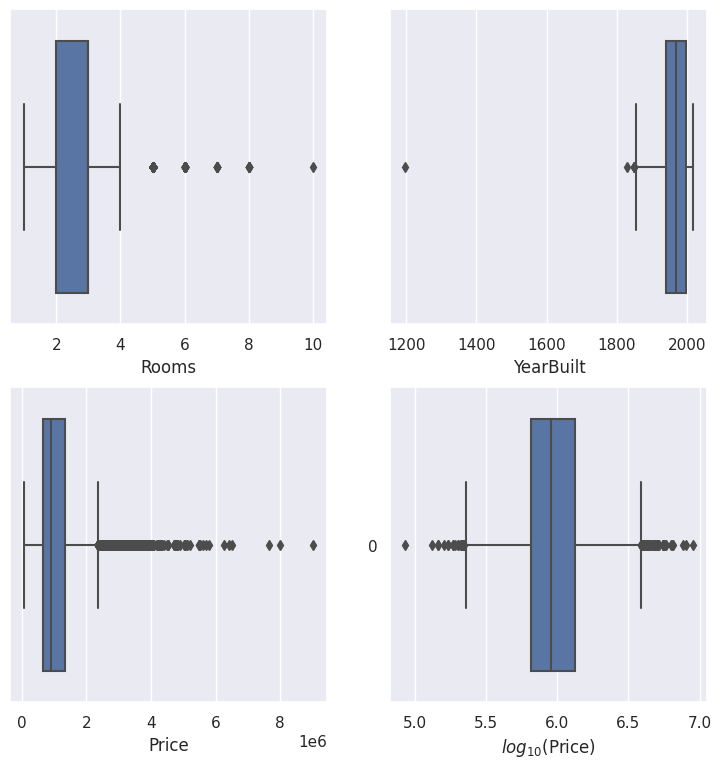
\includegraphics[width=1.0\columnwidth]{img/boxx4.png}
\caption{QQPLOT de Año de Construcción, Cantidad de Ambientes, Precio y del Precio en escala logarítmica.}
\label{box3}
\end{center}
\end{figure}

En resumen, se realizaron los cortes en 1,5 veces el Rango Intercuartilico, eliminando de esta manera los valores extremos en estas últimas variables analizadas. Finalmente nos queda de esta primera parte del entregable 2 una base de datos (\href{https://raw.githubusercontent.com/sebascoca/DiploDatos2023/main/AnalisisYCuracion/Practico/dfjoin.csv}{dfjoin.csv}) para comenzar con la Segunda Parte del análisis.

\clearpage

 \section*{Trabajo práctico entregable 2 - Parte 2}

En esta sección retomamos la tabla generada previamente: (\href{https://raw.githubusercontent.com/sebascoca/DiploDatos2023/main/AnalisisYCuracion/Practico/dfjoin.csv}{dfjoin.csv}). A partir de ésta, en esta parte del entregable, realizamos diferentes transformaciones a los datos, aplicando diversas técnicas. 

\subsection*{Dicotomización}
Las variables categóricas `Type' y `Regionname' fueron sometidas a la técnica ``one-hot encoding'' (codificación one-hot), la cual es utilizada en el procesamiento de datos y el aprendizaje automático para representar variables categóricas como vectores binarios. El one-hot encoding transforma cada categoría en una nueva columna binaria y asigna un valor de 1 en la columna correspondiente a la categoría y un valor de 0 en todas las demás columnas. Esto crea una representación numérica en la que se captura la información sobre la presencia o ausencia de cada categoría en un conjunto de datos. También se conoce este procedimiento como dumificación. Como resultado de ello se generaron 11 columnas nuevas: 3 de ellas para `Type' y 8 para `Regionnames'. 
También se generó un codificación binaria sobre las variables numéricas `Rooms' y `Price', realizando previamente la discretización ordinal de las mismas. O sea, se convirtió la variable continua en otra ordinal, segmentando sus valores en diferentes categorías o intervalos, de manera que cada categoría contenga aproximadamente la misma cantidad de observaciones.

\subsection*{Imputación}
Previa a la imputación es necesario realizar una representación gráfica para identificar cuales son las variables que presentan faltantes y en que proporción (Figuras \ref{faltantes} y \ref{faltantes2}).

\begin{figure} [!ht]
\begin{center}
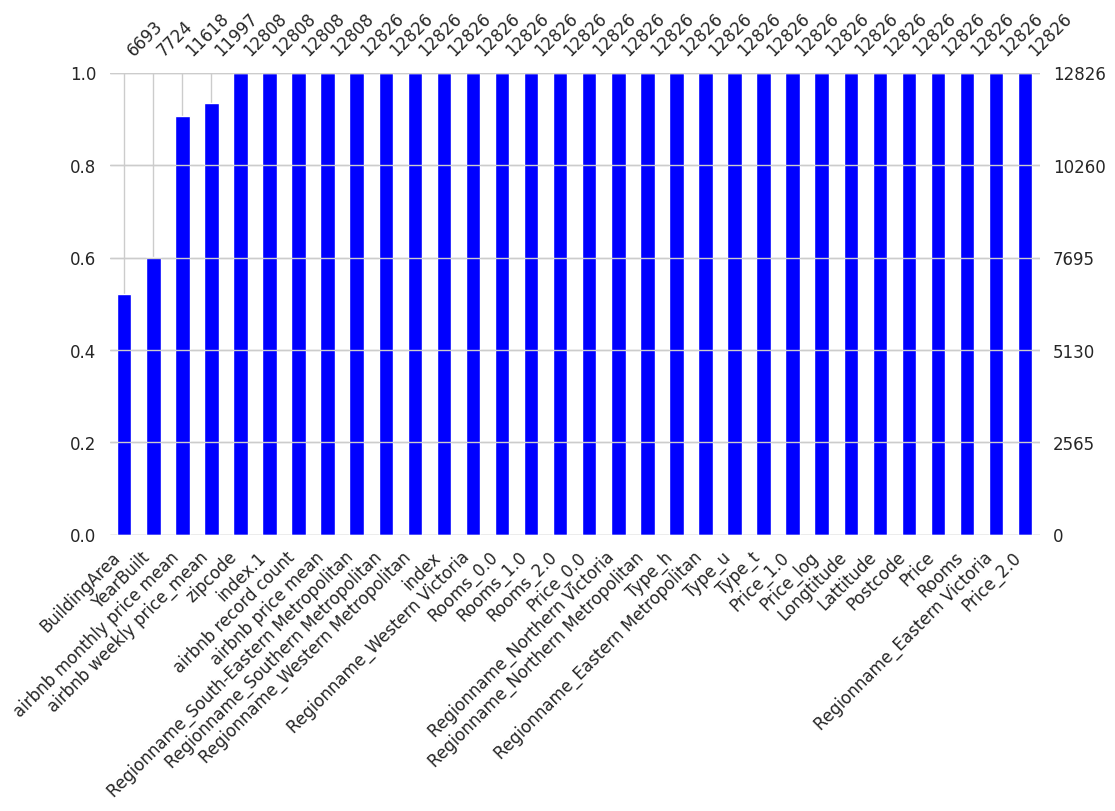
\includegraphics[width=1.0\columnwidth]{img/datosfaltantes.png}
\caption{Histograma Base completa - Visualización de Datos Faltantes.}
\label{faltantes}
\end{center}
\end{figure}

\begin{figure} [!ht]
\begin{center}
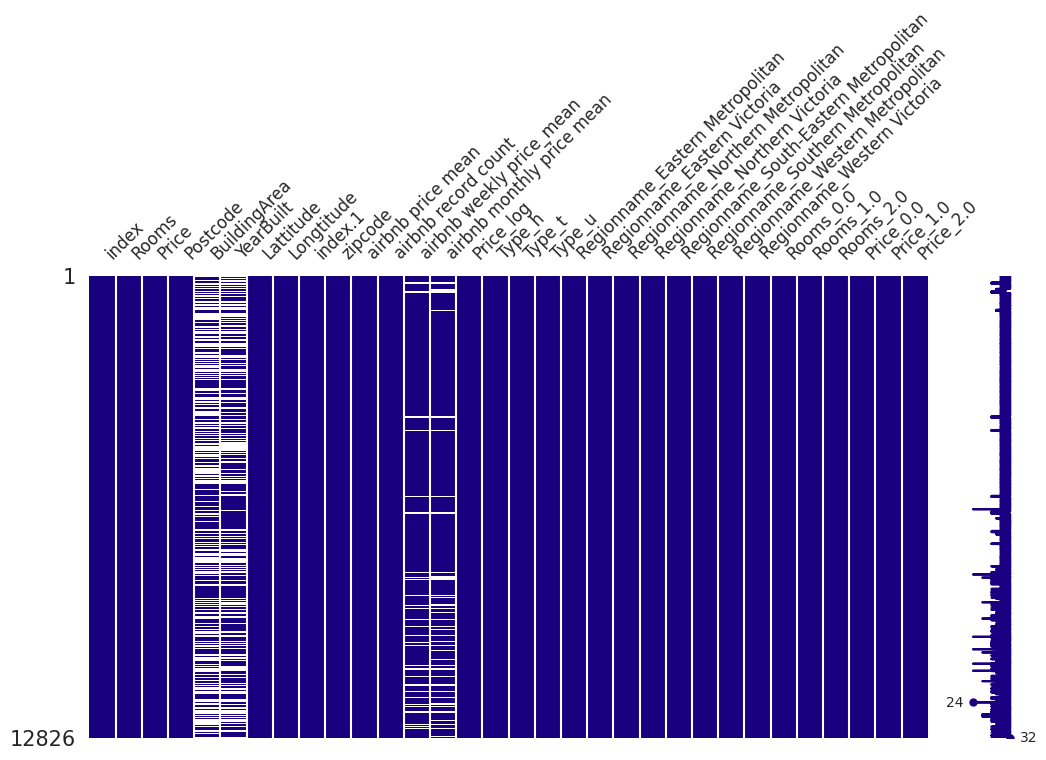
\includegraphics[width=1.0\columnwidth]{img/datosfaltantes2.png}
\caption{Histograma Base completa - Visualización individuos Faltantes.}
\label{faltantes2}
\end{center}
\end{figure}

En la Figura \ref{faltantes2}, se observa una correlación entre los datos faltantes de las variables "Building area" y "Year build", esto se debe a que existe una relación entre ellas, hay una tendencia en que las propiedades más nuevas tienen menos área de construcción.
Las variables `YearBuilt' y `BuildingArea' tienen numerosas entradas faltantes. La distribución original de datos tiene distribución bimodal, con un descenso en los registros alrededor de la década del '80, como se puede ver en la Figura \ref{f.imputacion}. El método KNN rellena los datos faltantes con valores entorno a este rango de años con vacíos de registros, dando lugar a una distribución unimodal en `YearBuilt'. 
Otro método explorado fue el Bayesian Ridge, el cual es una técnica flexible y efectiva que permite manejar datos incompletos de manera robusta. Sin embargo, es importante tener en cuenta que la calidad de las imputaciones depende de la calidad del modelo de regresión Ridge y de las suposiciones subyacentes sobre los datos. Para el caso particular de estudio, no fue satisfactorio el resultado dado que asignó valores erróneos como ser fechas futuras. No se modificó la naturaleza bimodal en el conjunto original de datos para `YearBuilt', estando concentradas las imputaciones para la década del '60 del siglo pasado. Por último, debemos destacar la inconsistencia en la imputación, lo cual queda reflejado por la ausencia de relación directa entre los valores asignados según KNN versus el método Bayesiano, como se puede ver en la Figura \ref{regresion}.

\begin{figure}[!t]
\begin{minipage}{0.48\textwidth}
  \centering
  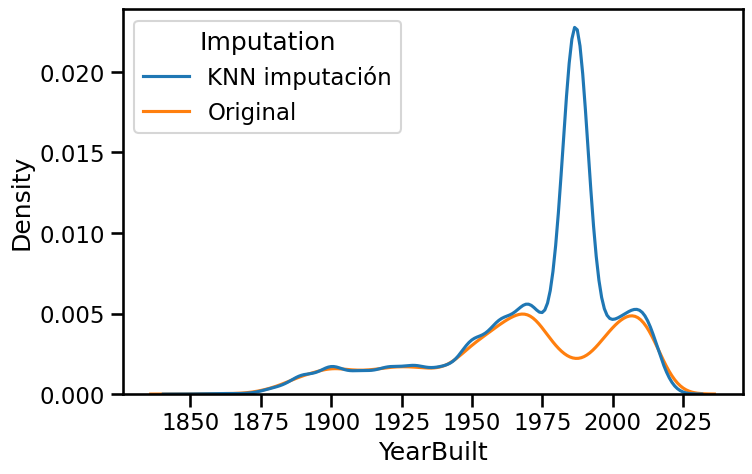
\includegraphics[width=\linewidth]{img/imputacion-KNN.png}
  %\caption{Distribución de densidad para la imputación KNN y su comparación con los datos originales.}
  %\label{fig:knn}
\end{minipage}\hfill
\begin{minipage}{0.48\textwidth}
  \centering
  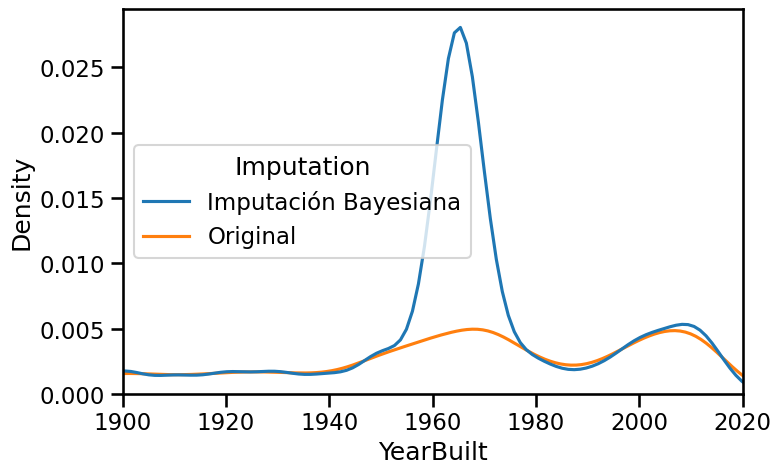
\includegraphics[width=\linewidth]{img/imputacion-bayesiana.png}
  %\caption{Distribución de densidad para la imputación Bayesiana y su comparación con los datos %originales.}
  %\label{fig:bayesiana}
\end{minipage}
\caption{Distribuciones de densidad para la imputación KNN (izquierda) y Bayesiana (derecha). Ambas comparadas con los datos originales en función del año de construcción.}
\label{f.imputacion}
\end{figure}



\begin{figure} [!t]
\begin{center}
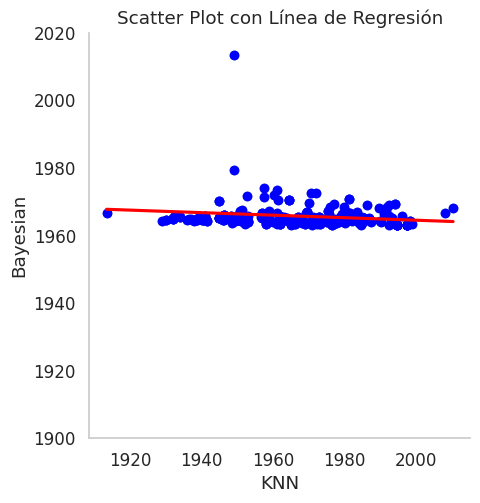
\includegraphics[width=0.4\columnwidth]{img/regresion.png}
\caption{Scatter plot donde se comparan ambas imputaciones, Bayesiana y KNN. Se presenta línea de regresión y se observa que no hay una relación directa entre las imputaciones.}
\label{regresion}
\end{center}
\end{figure}


\subsection*{Reducción de dimensionalidad}
Para realizar la reducción de dimensionalidad se aplicó un análisis de componentes principales o PCA sobre el conjunto completo de variables numéricas. Para ello previamente realizamos: (i) normalización por el rango en una escala continua \([-1, 1]\) y (ii) remoción de columnas irrelevantes para el problema. Los resultados indican existencia de redundancia en la información. Los primeros dos componentes lograron capturar la mitad de la varianza total contenida en los datos, como se puede ver en la Figura \ref{pca}.
Analizamos los scores de las viviendas a lo largo del eje 1 del PCA. También estudiamos su relación con el precio (a partir de su versión discretizada como variable ordinal). Puede verificarse que las viviendas más costosas se concentran en el dominio negativo del eje 1, siendo por lo tanto esta dimensión del PCA informativa con respecto al precio. Esto apunta en la dirección del objetivo primario de todo el trabajo: indagar acerca de la co-estructura entre rasgos de viviendas y precio.   

\begin{figure} [!t]
\begin{center}
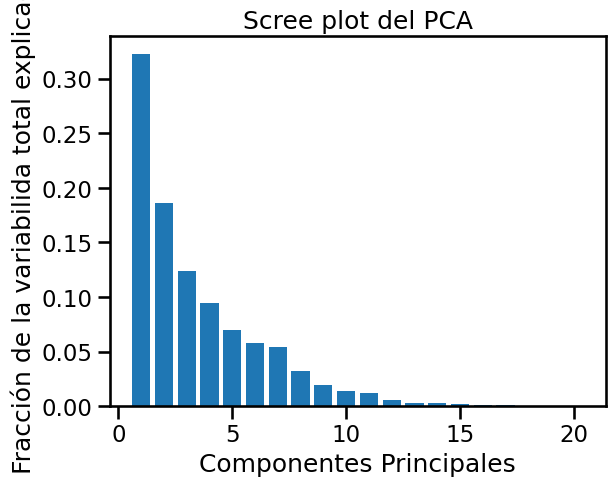
\includegraphics[width=0.6\columnwidth]{img/PCA.png}
\caption{Screeplot del Análisis de Componentes Principales (PCA). En el eje x del gráfico se representan los números de los componentes principales, mientras que en el eje y se muestra la varianza explicada}
\label{pca}
\end{center}
\end{figure}


\subsection*{Comentarios Finales}
Finalmente, luego de todas las transformaciones aplicadas en esta parte del entregable 2, se generó una tabla final que queda disponible en: \href{
https://raw.githubusercontent.com/sebascoca/DiploDatos2023/main/AnalisisYCuracion/Practico/tablafinalAEyC.csv}{tabla-final-AEyC.csv}. \\[.5cm]

Repositorio con todo el material: \href{https://github.com/sebascoca/DiploDatos2023/tree/main/AnalisisYCuracion/Practico}{GitHub del Práctico}



\end{document}





